% Options for packages loaded elsewhere
\PassOptionsToPackage{unicode}{hyperref}
\PassOptionsToPackage{hyphens}{url}
\PassOptionsToPackage{dvipsnames,svgnames,x11names}{xcolor}
%
\documentclass[
  letterpaper,
  DIV=11,
  numbers=noendperiod]{scrartcl}

\usepackage{amsmath,amssymb}
\usepackage{iftex}
\ifPDFTeX
  \usepackage[T1]{fontenc}
  \usepackage[utf8]{inputenc}
  \usepackage{textcomp} % provide euro and other symbols
\else % if luatex or xetex
  \usepackage{unicode-math}
  \defaultfontfeatures{Scale=MatchLowercase}
  \defaultfontfeatures[\rmfamily]{Ligatures=TeX,Scale=1}
\fi
\usepackage{lmodern}
\ifPDFTeX\else  
    % xetex/luatex font selection
\fi
% Use upquote if available, for straight quotes in verbatim environments
\IfFileExists{upquote.sty}{\usepackage{upquote}}{}
\IfFileExists{microtype.sty}{% use microtype if available
  \usepackage[]{microtype}
  \UseMicrotypeSet[protrusion]{basicmath} % disable protrusion for tt fonts
}{}
\makeatletter
\@ifundefined{KOMAClassName}{% if non-KOMA class
  \IfFileExists{parskip.sty}{%
    \usepackage{parskip}
  }{% else
    \setlength{\parindent}{0pt}
    \setlength{\parskip}{6pt plus 2pt minus 1pt}}
}{% if KOMA class
  \KOMAoptions{parskip=half}}
\makeatother
\usepackage{xcolor}
\setlength{\emergencystretch}{3em} % prevent overfull lines
\setcounter{secnumdepth}{-\maxdimen} % remove section numbering
% Make \paragraph and \subparagraph free-standing
\makeatletter
\ifx\paragraph\undefined\else
  \let\oldparagraph\paragraph
  \renewcommand{\paragraph}{
    \@ifstar
      \xxxParagraphStar
      \xxxParagraphNoStar
  }
  \newcommand{\xxxParagraphStar}[1]{\oldparagraph*{#1}\mbox{}}
  \newcommand{\xxxParagraphNoStar}[1]{\oldparagraph{#1}\mbox{}}
\fi
\ifx\subparagraph\undefined\else
  \let\oldsubparagraph\subparagraph
  \renewcommand{\subparagraph}{
    \@ifstar
      \xxxSubParagraphStar
      \xxxSubParagraphNoStar
  }
  \newcommand{\xxxSubParagraphStar}[1]{\oldsubparagraph*{#1}\mbox{}}
  \newcommand{\xxxSubParagraphNoStar}[1]{\oldsubparagraph{#1}\mbox{}}
\fi
\makeatother

\usepackage{color}
\usepackage{fancyvrb}
\newcommand{\VerbBar}{|}
\newcommand{\VERB}{\Verb[commandchars=\\\{\}]}
\DefineVerbatimEnvironment{Highlighting}{Verbatim}{commandchars=\\\{\}}
% Add ',fontsize=\small' for more characters per line
\usepackage{framed}
\definecolor{shadecolor}{RGB}{241,243,245}
\newenvironment{Shaded}{\begin{snugshade}}{\end{snugshade}}
\newcommand{\AlertTok}[1]{\textcolor[rgb]{0.68,0.00,0.00}{#1}}
\newcommand{\AnnotationTok}[1]{\textcolor[rgb]{0.37,0.37,0.37}{#1}}
\newcommand{\AttributeTok}[1]{\textcolor[rgb]{0.40,0.45,0.13}{#1}}
\newcommand{\BaseNTok}[1]{\textcolor[rgb]{0.68,0.00,0.00}{#1}}
\newcommand{\BuiltInTok}[1]{\textcolor[rgb]{0.00,0.23,0.31}{#1}}
\newcommand{\CharTok}[1]{\textcolor[rgb]{0.13,0.47,0.30}{#1}}
\newcommand{\CommentTok}[1]{\textcolor[rgb]{0.37,0.37,0.37}{#1}}
\newcommand{\CommentVarTok}[1]{\textcolor[rgb]{0.37,0.37,0.37}{\textit{#1}}}
\newcommand{\ConstantTok}[1]{\textcolor[rgb]{0.56,0.35,0.01}{#1}}
\newcommand{\ControlFlowTok}[1]{\textcolor[rgb]{0.00,0.23,0.31}{\textbf{#1}}}
\newcommand{\DataTypeTok}[1]{\textcolor[rgb]{0.68,0.00,0.00}{#1}}
\newcommand{\DecValTok}[1]{\textcolor[rgb]{0.68,0.00,0.00}{#1}}
\newcommand{\DocumentationTok}[1]{\textcolor[rgb]{0.37,0.37,0.37}{\textit{#1}}}
\newcommand{\ErrorTok}[1]{\textcolor[rgb]{0.68,0.00,0.00}{#1}}
\newcommand{\ExtensionTok}[1]{\textcolor[rgb]{0.00,0.23,0.31}{#1}}
\newcommand{\FloatTok}[1]{\textcolor[rgb]{0.68,0.00,0.00}{#1}}
\newcommand{\FunctionTok}[1]{\textcolor[rgb]{0.28,0.35,0.67}{#1}}
\newcommand{\ImportTok}[1]{\textcolor[rgb]{0.00,0.46,0.62}{#1}}
\newcommand{\InformationTok}[1]{\textcolor[rgb]{0.37,0.37,0.37}{#1}}
\newcommand{\KeywordTok}[1]{\textcolor[rgb]{0.00,0.23,0.31}{\textbf{#1}}}
\newcommand{\NormalTok}[1]{\textcolor[rgb]{0.00,0.23,0.31}{#1}}
\newcommand{\OperatorTok}[1]{\textcolor[rgb]{0.37,0.37,0.37}{#1}}
\newcommand{\OtherTok}[1]{\textcolor[rgb]{0.00,0.23,0.31}{#1}}
\newcommand{\PreprocessorTok}[1]{\textcolor[rgb]{0.68,0.00,0.00}{#1}}
\newcommand{\RegionMarkerTok}[1]{\textcolor[rgb]{0.00,0.23,0.31}{#1}}
\newcommand{\SpecialCharTok}[1]{\textcolor[rgb]{0.37,0.37,0.37}{#1}}
\newcommand{\SpecialStringTok}[1]{\textcolor[rgb]{0.13,0.47,0.30}{#1}}
\newcommand{\StringTok}[1]{\textcolor[rgb]{0.13,0.47,0.30}{#1}}
\newcommand{\VariableTok}[1]{\textcolor[rgb]{0.07,0.07,0.07}{#1}}
\newcommand{\VerbatimStringTok}[1]{\textcolor[rgb]{0.13,0.47,0.30}{#1}}
\newcommand{\WarningTok}[1]{\textcolor[rgb]{0.37,0.37,0.37}{\textit{#1}}}

\providecommand{\tightlist}{%
  \setlength{\itemsep}{0pt}\setlength{\parskip}{0pt}}\usepackage{longtable,booktabs,array}
\usepackage{calc} % for calculating minipage widths
% Correct order of tables after \paragraph or \subparagraph
\usepackage{etoolbox}
\makeatletter
\patchcmd\longtable{\par}{\if@noskipsec\mbox{}\fi\par}{}{}
\makeatother
% Allow footnotes in longtable head/foot
\IfFileExists{footnotehyper.sty}{\usepackage{footnotehyper}}{\usepackage{footnote}}
\makesavenoteenv{longtable}
\usepackage{graphicx}
\makeatletter
\def\maxwidth{\ifdim\Gin@nat@width>\linewidth\linewidth\else\Gin@nat@width\fi}
\def\maxheight{\ifdim\Gin@nat@height>\textheight\textheight\else\Gin@nat@height\fi}
\makeatother
% Scale images if necessary, so that they will not overflow the page
% margins by default, and it is still possible to overwrite the defaults
% using explicit options in \includegraphics[width, height, ...]{}
\setkeys{Gin}{width=\maxwidth,height=\maxheight,keepaspectratio}
% Set default figure placement to htbp
\makeatletter
\def\fps@figure{htbp}
\makeatother

\usepackage{fontspec}
\usepackage{multirow}
\usepackage{multicol}
\usepackage{colortbl}
\usepackage{hhline}
\newlength\Oldarrayrulewidth
\newlength\Oldtabcolsep
\usepackage{longtable}
\usepackage{array}
\usepackage{hyperref}
\usepackage{float}
\usepackage{wrapfig}
\KOMAoption{captions}{tableheading}
\makeatletter
\@ifpackageloaded{caption}{}{\usepackage{caption}}
\AtBeginDocument{%
\ifdefined\contentsname
  \renewcommand*\contentsname{Table of contents}
\else
  \newcommand\contentsname{Table of contents}
\fi
\ifdefined\listfigurename
  \renewcommand*\listfigurename{List of Figures}
\else
  \newcommand\listfigurename{List of Figures}
\fi
\ifdefined\listtablename
  \renewcommand*\listtablename{List of Tables}
\else
  \newcommand\listtablename{List of Tables}
\fi
\ifdefined\figurename
  \renewcommand*\figurename{Figure}
\else
  \newcommand\figurename{Figure}
\fi
\ifdefined\tablename
  \renewcommand*\tablename{Table}
\else
  \newcommand\tablename{Table}
\fi
}
\@ifpackageloaded{float}{}{\usepackage{float}}
\floatstyle{ruled}
\@ifundefined{c@chapter}{\newfloat{codelisting}{h}{lop}}{\newfloat{codelisting}{h}{lop}[chapter]}
\floatname{codelisting}{Listing}
\newcommand*\listoflistings{\listof{codelisting}{List of Listings}}
\makeatother
\makeatletter
\makeatother
\makeatletter
\@ifpackageloaded{caption}{}{\usepackage{caption}}
\@ifpackageloaded{subcaption}{}{\usepackage{subcaption}}
\makeatother

\ifLuaTeX
  \usepackage{selnolig}  % disable illegal ligatures
\fi
\usepackage{bookmark}

\IfFileExists{xurl.sty}{\usepackage{xurl}}{} % add URL line breaks if available
\urlstyle{same} % disable monospaced font for URLs
\hypersetup{
  pdftitle={Untitled},
  colorlinks=true,
  linkcolor={blue},
  filecolor={Maroon},
  citecolor={Blue},
  urlcolor={Blue},
  pdfcreator={LaTeX via pandoc}}


\title{Untitled}
\author{}
\date{}

\begin{document}
\maketitle


\subsection{Homework 3}\label{homework-3}

\section{Part 1. Setup}\label{part-1.-setup}

\begin{Shaded}
\begin{Highlighting}[]
\CommentTok{\# read in libraries}
\FunctionTok{library}\NormalTok{(tidyverse)}
\FunctionTok{library}\NormalTok{(here)}
\FunctionTok{library}\NormalTok{(flextable)}
\FunctionTok{library}\NormalTok{(janitor)}
\FunctionTok{library}\NormalTok{(readxl)}
\FunctionTok{library}\NormalTok{(officer)}

\CommentTok{\# read in personal data}
\NormalTok{mydata }\OtherTok{\textless{}{-}} \FunctionTok{read\_csv}\NormalTok{(here}\SpecialCharTok{::}\FunctionTok{here}\NormalTok{(}\StringTok{"data"}\NormalTok{, }\StringTok{"Personal Data Project {-} Sheet1.csv"}\NormalTok{))}
\end{Highlighting}
\end{Shaded}

\section{Part 2. Problems}\label{part-2.-problems}

\subsection{a.}\label{a.}

To summarize the data and compare a response variable between
categories, I will calculate the median pages per minute, by dividing
the numbers of pages read by the total time of the read, for each
session to compare reading effectiveness across different locations.
This comparison would be informative because different environments
might offer varying levels of comfort, light, or distraction which could
impact my focus, and consequently, how well I understood the material.

\subsection{b.}\label{b.}

\begin{Shaded}
\begin{Highlighting}[]
\NormalTok{df }\OtherTok{\textless{}{-}} \FunctionTok{clean\_names}\NormalTok{(mydata) }\SpecialCharTok{|\textgreater{}} \CommentTok{\# clean column names}
  \CommentTok{\# adding pages\_per\_minute column}
  \FunctionTok{mutate}\NormalTok{(}\AttributeTok{pages\_per\_minute =} \FunctionTok{ifelse}\NormalTok{(total\_time\_of\_reading }\SpecialCharTok{\textgreater{}} \DecValTok{0}\NormalTok{,  number\_of\_pages }\SpecialCharTok{/}\NormalTok{ total\_time\_of\_reading, }\DecValTok{0}\NormalTok{))}

\NormalTok{df\_summary }\OtherTok{\textless{}{-}}\NormalTok{ df }\SpecialCharTok{|\textgreater{}} \CommentTok{\# create new data frame for mean pages per minute}
  \FunctionTok{group\_by}\NormalTok{(location) }\SpecialCharTok{|\textgreater{}} \CommentTok{\# group by location}
  \FunctionTok{summarise}\NormalTok{(}
    \AttributeTok{N =} \FunctionTok{n}\NormalTok{(),                               }\CommentTok{\# Count of observations in each group}
    \AttributeTok{Mean\_PPM =} \FunctionTok{mean}\NormalTok{(pages\_per\_minute, }\AttributeTok{na.rm =} \ConstantTok{TRUE}\NormalTok{),    }\CommentTok{\# Mean Pages Per Minute}
    \AttributeTok{Median\_PPM =} \FunctionTok{median}\NormalTok{(pages\_per\_minute, }\AttributeTok{na.rm =} \ConstantTok{TRUE}\NormalTok{), }\CommentTok{\# Median Pages Per Minute}
    \AttributeTok{SD\_PPM =} \FunctionTok{sd}\NormalTok{(pages\_per\_minute, }\AttributeTok{na.rm =} \ConstantTok{TRUE}\NormalTok{),        }\CommentTok{\# Standard Deviation of PPM}
    \AttributeTok{IQR\_PPM =} \FunctionTok{IQR}\NormalTok{(pages\_per\_minute, }\AttributeTok{na.rm =} \ConstantTok{TRUE}\NormalTok{),      }\CommentTok{\# Interquartile Range of PPM}
    \AttributeTok{Min\_PPM =} \FunctionTok{min}\NormalTok{(pages\_per\_minute, }\AttributeTok{na.rm =} \ConstantTok{TRUE}\NormalTok{),      }\CommentTok{\# Minimum PPM}
    \AttributeTok{Max\_PPM =} \FunctionTok{max}\NormalTok{(pages\_per\_minute, }\AttributeTok{na.rm =} \ConstantTok{TRUE}\NormalTok{)) }\CommentTok{\# calculate the mean}

\FunctionTok{ggplot}\NormalTok{(df, }\CommentTok{\# plotting the data}
       \FunctionTok{aes}\NormalTok{(}\AttributeTok{x =}\NormalTok{ location, }\CommentTok{\# location on x axis}
               \AttributeTok{y =}\NormalTok{ pages\_per\_minute)) }\SpecialCharTok{+} \CommentTok{\# Pages per minute on the y axis}
         \FunctionTok{geom\_boxplot}\NormalTok{(}\FunctionTok{aes}\NormalTok{(}\AttributeTok{fill =}\NormalTok{ location)) }\SpecialCharTok{+} \CommentTok{\# creating boxplot}
  \FunctionTok{geom\_jitter}\NormalTok{(}\AttributeTok{width =} \FloatTok{0.2}\NormalTok{, }\AttributeTok{size =} \DecValTok{1}\NormalTok{, }\AttributeTok{color =} \StringTok{"black"}\NormalTok{, }\AttributeTok{alpha =} \FloatTok{0.7}\NormalTok{) }\SpecialCharTok{+} \CommentTok{\# adding the underlying data}
  \FunctionTok{scale\_fill\_manual}\NormalTok{(}\AttributeTok{values =} \FunctionTok{c}\NormalTok{( }\CommentTok{\# add different colors than default}
    \StringTok{"Balcony"} \OtherTok{=} \StringTok{"\#1f77b4"}\NormalTok{, }\CommentTok{\# blue for balcony}
    \StringTok{"Bed"} \OtherTok{=} \StringTok{"\#ff7f0e"} \CommentTok{\# orange for bed}
\NormalTok{  )) }\SpecialCharTok{+}
  \FunctionTok{theme\_bw}\NormalTok{() }\SpecialCharTok{+} \CommentTok{\# add theme for aesthetics}
  \FunctionTok{labs}\NormalTok{( }\CommentTok{\# label function to rename labels}
    \AttributeTok{x =} \StringTok{"Reading Location"}\NormalTok{, }\CommentTok{\# new x axis title}
    \AttributeTok{y =} \StringTok{"Pages Per Minute"}\NormalTok{, }\CommentTok{\# new y axis title}
    \AttributeTok{title =} \StringTok{"Reading Efficiency (Pages Per Minute) by Location"} \CommentTok{\# title for visualization}
\NormalTok{  )}
\end{Highlighting}
\end{Shaded}

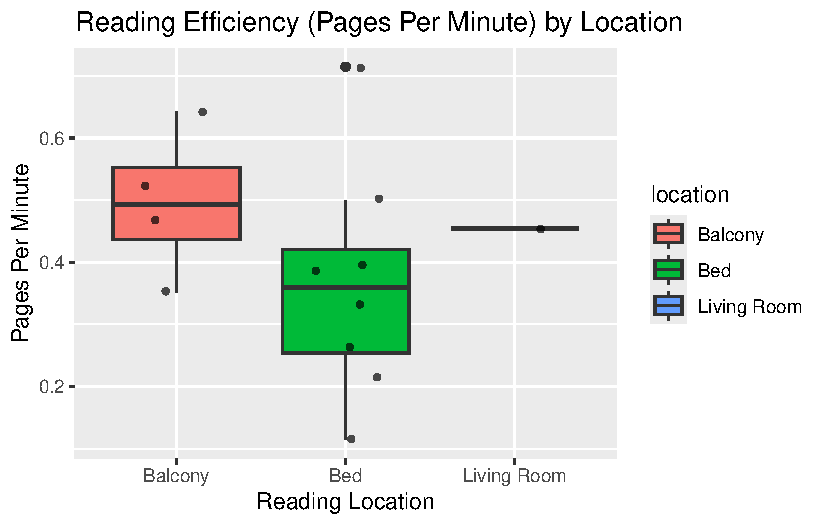
\includegraphics{Untitled_files/figure-pdf/unnamed-chunk-2-1.pdf}

\subsection{c.}\label{c.}

Figure 1. Reading Efficiency (Pages Per Minute) by Location. Box plots
display the distribution and summary statistics of reading efficiency at
two locations: the balcony and the bed. While both locations show
similar median reading speeds, the balcony shows a tighter distribution
compared to the wider spread of values observed for reading in bed.

\subsection{d.}\label{d.}

\begin{Shaded}
\begin{Highlighting}[]
\NormalTok{table1 }\OtherTok{\textless{}{-}} \FunctionTok{flextable}\NormalTok{(df\_summary) }\SpecialCharTok{|\textgreater{}} \CommentTok{\# create table using flextable}
  \FunctionTok{colformat\_double}\NormalTok{(}\AttributeTok{digits =} \DecValTok{2}\NormalTok{) }\SpecialCharTok{|\textgreater{}} \CommentTok{\# rounding to nearest decimal}
  \FunctionTok{set\_header\_labels}\NormalTok{( }\CommentTok{\# changing header labels}
    \AttributeTok{location =} \StringTok{"Location"}\NormalTok{, }\CommentTok{\# capitalize location}
    \AttributeTok{N =} \StringTok{"Count"}\NormalTok{, }\CommentTok{\# cleaning the header names}
    \AttributeTok{Mean\_PPM =} \StringTok{"Mean PPM"}\NormalTok{,}
    \AttributeTok{Median\_PPM =} \StringTok{"Median PPM"}\NormalTok{,}
    \AttributeTok{SD\_PPM =} \StringTok{"Std. Dev. PPM"}\NormalTok{,}
    \AttributeTok{IQR\_PPM =} \StringTok{"IQR PPM"}\NormalTok{,}
    \AttributeTok{Min\_PPM =} \StringTok{"Min PPM"}\NormalTok{,}
    \AttributeTok{Max\_PPM =} \StringTok{"Max PPM"}
\NormalTok{  ) }\SpecialCharTok{|\textgreater{}}
  \FunctionTok{autofit}\NormalTok{() }\SpecialCharTok{|\textgreater{}} \CommentTok{\# autofit function to make everything fit}
  \FunctionTok{theme\_zebra}\NormalTok{() }\SpecialCharTok{|\textgreater{}} \CommentTok{\# theme}
  \FunctionTok{align}\NormalTok{(}\AttributeTok{align =} \StringTok{"center"}\NormalTok{, }\AttributeTok{part =} \StringTok{"all"}\NormalTok{) }\SpecialCharTok{|\textgreater{}} \CommentTok{\# center align all parts of the table}
  \FunctionTok{border\_outer}\NormalTok{(}\AttributeTok{border =} \FunctionTok{fp\_border}\NormalTok{(}\AttributeTok{color =} \StringTok{"black"}\NormalTok{, }\AttributeTok{width =} \DecValTok{2}\NormalTok{)) }\SpecialCharTok{|\textgreater{}} \CommentTok{\# adding outer border}
  \FunctionTok{border\_inner}\NormalTok{(}\AttributeTok{border =} \FunctionTok{fp\_border}\NormalTok{(}\AttributeTok{color =} \StringTok{"grey"}\NormalTok{, }\AttributeTok{width =} \DecValTok{1}\NormalTok{)) }\CommentTok{\# adding inner border}

\NormalTok{table1 }\CommentTok{\# displaying the table}
\end{Highlighting}
\end{Shaded}

\global\setlength{\Oldarrayrulewidth}{\arrayrulewidth}

\global\setlength{\Oldtabcolsep}{\tabcolsep}

\setlength{\tabcolsep}{2pt}

\renewcommand*{\arraystretch}{1.5}



\providecommand{\ascline}[3]{\noalign{\global\arrayrulewidth #1}\arrayrulecolor[HTML]{#2}\cline{#3}}

\begin{longtable*}[c]{|p{0.86in}|p{0.69in}|p{1.04in}|p{1.16in}|p{1.29in}|p{0.93in}|p{0.90in}|p{0.95in}}



\hhline{>{\arrayrulecolor[HTML]{000000}\global\arrayrulewidth=2pt}->{\arrayrulecolor[HTML]{000000}\global\arrayrulewidth=2pt}->{\arrayrulecolor[HTML]{000000}\global\arrayrulewidth=2pt}->{\arrayrulecolor[HTML]{000000}\global\arrayrulewidth=2pt}->{\arrayrulecolor[HTML]{000000}\global\arrayrulewidth=2pt}->{\arrayrulecolor[HTML]{000000}\global\arrayrulewidth=2pt}->{\arrayrulecolor[HTML]{000000}\global\arrayrulewidth=2pt}->{\arrayrulecolor[HTML]{000000}\global\arrayrulewidth=2pt}-}

\multicolumn{1}{!{\color[HTML]{000000}\vrule width 2pt}>{\cellcolor[HTML]{CFCFCF}\centering}m{\dimexpr 0.86in+0\tabcolsep}}{\textcolor[HTML]{000000}{\fontsize{11}{11}\selectfont{\global\setmainfont{Helvetica}{\textbf{Location}}}}} & \multicolumn{1}{!{\color[HTML]{BEBEBE}\vrule width 1pt}>{\cellcolor[HTML]{CFCFCF}\centering}m{\dimexpr 0.69in+0\tabcolsep}}{\textcolor[HTML]{000000}{\fontsize{11}{11}\selectfont{\global\setmainfont{Helvetica}{\textbf{Count}}}}} & \multicolumn{1}{!{\color[HTML]{BEBEBE}\vrule width 1pt}>{\cellcolor[HTML]{CFCFCF}\centering}m{\dimexpr 1.04in+0\tabcolsep}}{\textcolor[HTML]{000000}{\fontsize{11}{11}\selectfont{\global\setmainfont{Helvetica}{\textbf{Mean\ PPM}}}}} & \multicolumn{1}{!{\color[HTML]{BEBEBE}\vrule width 1pt}>{\cellcolor[HTML]{CFCFCF}\centering}m{\dimexpr 1.16in+0\tabcolsep}}{\textcolor[HTML]{000000}{\fontsize{11}{11}\selectfont{\global\setmainfont{Helvetica}{\textbf{Median\ PPM}}}}} & \multicolumn{1}{!{\color[HTML]{BEBEBE}\vrule width 1pt}>{\cellcolor[HTML]{CFCFCF}\centering}m{\dimexpr 1.29in+0\tabcolsep}}{\textcolor[HTML]{000000}{\fontsize{11}{11}\selectfont{\global\setmainfont{Helvetica}{\textbf{Std.\ Dev.\ PPM}}}}} & \multicolumn{1}{!{\color[HTML]{BEBEBE}\vrule width 1pt}>{\cellcolor[HTML]{CFCFCF}\centering}m{\dimexpr 0.93in+0\tabcolsep}}{\textcolor[HTML]{000000}{\fontsize{11}{11}\selectfont{\global\setmainfont{Helvetica}{\textbf{IQR\ PPM}}}}} & \multicolumn{1}{!{\color[HTML]{BEBEBE}\vrule width 1pt}>{\cellcolor[HTML]{CFCFCF}\centering}m{\dimexpr 0.9in+0\tabcolsep}}{\textcolor[HTML]{000000}{\fontsize{11}{11}\selectfont{\global\setmainfont{Helvetica}{\textbf{Min\ PPM}}}}} & \multicolumn{1}{!{\color[HTML]{BEBEBE}\vrule width 1pt}>{\cellcolor[HTML]{CFCFCF}\centering}m{\dimexpr 0.95in+0\tabcolsep}!{\color[HTML]{000000}\vrule width 2pt}}{\textcolor[HTML]{000000}{\fontsize{11}{11}\selectfont{\global\setmainfont{Helvetica}{\textbf{Max\ PPM}}}}} \\

\noalign{\global\arrayrulewidth 2pt}\arrayrulecolor[HTML]{000000}

\hhline{|>{\arrayrulecolor[HTML]{000000}\global\arrayrulewidth=2pt}-|>{\arrayrulecolor[HTML]{000000}\global\arrayrulewidth=2pt}-|>{\arrayrulecolor[HTML]{000000}\global\arrayrulewidth=2pt}-|>{\arrayrulecolor[HTML]{000000}\global\arrayrulewidth=2pt}-|>{\arrayrulecolor[HTML]{000000}\global\arrayrulewidth=2pt}-|>{\arrayrulecolor[HTML]{000000}\global\arrayrulewidth=2pt}-|>{\arrayrulecolor[HTML]{000000}\global\arrayrulewidth=2pt}-|>{\arrayrulecolor[HTML]{000000}\global\arrayrulewidth=2pt}-}\endfirsthead 

\hhline{>{\arrayrulecolor[HTML]{000000}\global\arrayrulewidth=2pt}->{\arrayrulecolor[HTML]{000000}\global\arrayrulewidth=2pt}->{\arrayrulecolor[HTML]{000000}\global\arrayrulewidth=2pt}->{\arrayrulecolor[HTML]{000000}\global\arrayrulewidth=2pt}->{\arrayrulecolor[HTML]{000000}\global\arrayrulewidth=2pt}->{\arrayrulecolor[HTML]{000000}\global\arrayrulewidth=2pt}->{\arrayrulecolor[HTML]{000000}\global\arrayrulewidth=2pt}->{\arrayrulecolor[HTML]{000000}\global\arrayrulewidth=2pt}-}

\multicolumn{1}{!{\color[HTML]{000000}\vrule width 2pt}>{\cellcolor[HTML]{CFCFCF}\centering}m{\dimexpr 0.86in+0\tabcolsep}}{\textcolor[HTML]{000000}{\fontsize{11}{11}\selectfont{\global\setmainfont{Helvetica}{\textbf{Location}}}}} & \multicolumn{1}{!{\color[HTML]{BEBEBE}\vrule width 1pt}>{\cellcolor[HTML]{CFCFCF}\centering}m{\dimexpr 0.69in+0\tabcolsep}}{\textcolor[HTML]{000000}{\fontsize{11}{11}\selectfont{\global\setmainfont{Helvetica}{\textbf{Count}}}}} & \multicolumn{1}{!{\color[HTML]{BEBEBE}\vrule width 1pt}>{\cellcolor[HTML]{CFCFCF}\centering}m{\dimexpr 1.04in+0\tabcolsep}}{\textcolor[HTML]{000000}{\fontsize{11}{11}\selectfont{\global\setmainfont{Helvetica}{\textbf{Mean\ PPM}}}}} & \multicolumn{1}{!{\color[HTML]{BEBEBE}\vrule width 1pt}>{\cellcolor[HTML]{CFCFCF}\centering}m{\dimexpr 1.16in+0\tabcolsep}}{\textcolor[HTML]{000000}{\fontsize{11}{11}\selectfont{\global\setmainfont{Helvetica}{\textbf{Median\ PPM}}}}} & \multicolumn{1}{!{\color[HTML]{BEBEBE}\vrule width 1pt}>{\cellcolor[HTML]{CFCFCF}\centering}m{\dimexpr 1.29in+0\tabcolsep}}{\textcolor[HTML]{000000}{\fontsize{11}{11}\selectfont{\global\setmainfont{Helvetica}{\textbf{Std.\ Dev.\ PPM}}}}} & \multicolumn{1}{!{\color[HTML]{BEBEBE}\vrule width 1pt}>{\cellcolor[HTML]{CFCFCF}\centering}m{\dimexpr 0.93in+0\tabcolsep}}{\textcolor[HTML]{000000}{\fontsize{11}{11}\selectfont{\global\setmainfont{Helvetica}{\textbf{IQR\ PPM}}}}} & \multicolumn{1}{!{\color[HTML]{BEBEBE}\vrule width 1pt}>{\cellcolor[HTML]{CFCFCF}\centering}m{\dimexpr 0.9in+0\tabcolsep}}{\textcolor[HTML]{000000}{\fontsize{11}{11}\selectfont{\global\setmainfont{Helvetica}{\textbf{Min\ PPM}}}}} & \multicolumn{1}{!{\color[HTML]{BEBEBE}\vrule width 1pt}>{\cellcolor[HTML]{CFCFCF}\centering}m{\dimexpr 0.95in+0\tabcolsep}!{\color[HTML]{000000}\vrule width 2pt}}{\textcolor[HTML]{000000}{\fontsize{11}{11}\selectfont{\global\setmainfont{Helvetica}{\textbf{Max\ PPM}}}}} \\

\noalign{\global\arrayrulewidth 2pt}\arrayrulecolor[HTML]{000000}

\hhline{|>{\arrayrulecolor[HTML]{000000}\global\arrayrulewidth=2pt}-|>{\arrayrulecolor[HTML]{000000}\global\arrayrulewidth=2pt}-|>{\arrayrulecolor[HTML]{000000}\global\arrayrulewidth=2pt}-|>{\arrayrulecolor[HTML]{000000}\global\arrayrulewidth=2pt}-|>{\arrayrulecolor[HTML]{000000}\global\arrayrulewidth=2pt}-|>{\arrayrulecolor[HTML]{000000}\global\arrayrulewidth=2pt}-|>{\arrayrulecolor[HTML]{000000}\global\arrayrulewidth=2pt}-|>{\arrayrulecolor[HTML]{000000}\global\arrayrulewidth=2pt}-}\endhead



\multicolumn{1}{!{\color[HTML]{000000}\vrule width 2pt}>{\cellcolor[HTML]{EFEFEF}\centering}m{\dimexpr 0.86in+0\tabcolsep}}{\textcolor[HTML]{000000}{\fontsize{11}{11}\selectfont{\global\setmainfont{Helvetica}{Balcony}}}} & \multicolumn{1}{!{\color[HTML]{BEBEBE}\vrule width 1pt}>{\cellcolor[HTML]{EFEFEF}\centering}m{\dimexpr 0.69in+0\tabcolsep}}{\textcolor[HTML]{000000}{\fontsize{11}{11}\selectfont{\global\setmainfont{Helvetica}{4}}}} & \multicolumn{1}{!{\color[HTML]{BEBEBE}\vrule width 1pt}>{\cellcolor[HTML]{EFEFEF}\centering}m{\dimexpr 1.04in+0\tabcolsep}}{\textcolor[HTML]{000000}{\fontsize{11}{11}\selectfont{\global\setmainfont{Helvetica}{0.50}}}} & \multicolumn{1}{!{\color[HTML]{BEBEBE}\vrule width 1pt}>{\cellcolor[HTML]{EFEFEF}\centering}m{\dimexpr 1.16in+0\tabcolsep}}{\textcolor[HTML]{000000}{\fontsize{11}{11}\selectfont{\global\setmainfont{Helvetica}{0.49}}}} & \multicolumn{1}{!{\color[HTML]{BEBEBE}\vrule width 1pt}>{\cellcolor[HTML]{EFEFEF}\centering}m{\dimexpr 1.29in+0\tabcolsep}}{\textcolor[HTML]{000000}{\fontsize{11}{11}\selectfont{\global\setmainfont{Helvetica}{0.12}}}} & \multicolumn{1}{!{\color[HTML]{BEBEBE}\vrule width 1pt}>{\cellcolor[HTML]{EFEFEF}\centering}m{\dimexpr 0.93in+0\tabcolsep}}{\textcolor[HTML]{000000}{\fontsize{11}{11}\selectfont{\global\setmainfont{Helvetica}{0.12}}}} & \multicolumn{1}{!{\color[HTML]{BEBEBE}\vrule width 1pt}>{\cellcolor[HTML]{EFEFEF}\centering}m{\dimexpr 0.9in+0\tabcolsep}}{\textcolor[HTML]{000000}{\fontsize{11}{11}\selectfont{\global\setmainfont{Helvetica}{0.35}}}} & \multicolumn{1}{!{\color[HTML]{BEBEBE}\vrule width 1pt}>{\cellcolor[HTML]{EFEFEF}\centering}m{\dimexpr 0.95in+0\tabcolsep}!{\color[HTML]{000000}\vrule width 2pt}}{\textcolor[HTML]{000000}{\fontsize{11}{11}\selectfont{\global\setmainfont{Helvetica}{0.64}}}} \\

\noalign{\global\arrayrulewidth 2pt}\arrayrulecolor[HTML]{000000}

\hhline{|>{\arrayrulecolor[HTML]{BEBEBE}\global\arrayrulewidth=1pt}-|>{\arrayrulecolor[HTML]{BEBEBE}\global\arrayrulewidth=1pt}-|>{\arrayrulecolor[HTML]{BEBEBE}\global\arrayrulewidth=1pt}-|>{\arrayrulecolor[HTML]{BEBEBE}\global\arrayrulewidth=1pt}-|>{\arrayrulecolor[HTML]{BEBEBE}\global\arrayrulewidth=1pt}-|>{\arrayrulecolor[HTML]{BEBEBE}\global\arrayrulewidth=1pt}-|>{\arrayrulecolor[HTML]{BEBEBE}\global\arrayrulewidth=1pt}-|>{\arrayrulecolor[HTML]{BEBEBE}\global\arrayrulewidth=1pt}-}



\multicolumn{1}{!{\color[HTML]{000000}\vrule width 2pt}>{\centering}m{\dimexpr 0.86in+0\tabcolsep}}{\textcolor[HTML]{000000}{\fontsize{11}{11}\selectfont{\global\setmainfont{Helvetica}{Bed}}}} & \multicolumn{1}{!{\color[HTML]{BEBEBE}\vrule width 1pt}>{\centering}m{\dimexpr 0.69in+0\tabcolsep}}{\textcolor[HTML]{000000}{\fontsize{11}{11}\selectfont{\global\setmainfont{Helvetica}{8}}}} & \multicolumn{1}{!{\color[HTML]{BEBEBE}\vrule width 1pt}>{\centering}m{\dimexpr 1.04in+0\tabcolsep}}{\textcolor[HTML]{000000}{\fontsize{11}{11}\selectfont{\global\setmainfont{Helvetica}{0.37}}}} & \multicolumn{1}{!{\color[HTML]{BEBEBE}\vrule width 1pt}>{\centering}m{\dimexpr 1.16in+0\tabcolsep}}{\textcolor[HTML]{000000}{\fontsize{11}{11}\selectfont{\global\setmainfont{Helvetica}{0.36}}}} & \multicolumn{1}{!{\color[HTML]{BEBEBE}\vrule width 1pt}>{\centering}m{\dimexpr 1.29in+0\tabcolsep}}{\textcolor[HTML]{000000}{\fontsize{11}{11}\selectfont{\global\setmainfont{Helvetica}{0.18}}}} & \multicolumn{1}{!{\color[HTML]{BEBEBE}\vrule width 1pt}>{\centering}m{\dimexpr 0.93in+0\tabcolsep}}{\textcolor[HTML]{000000}{\fontsize{11}{11}\selectfont{\global\setmainfont{Helvetica}{0.17}}}} & \multicolumn{1}{!{\color[HTML]{BEBEBE}\vrule width 1pt}>{\centering}m{\dimexpr 0.9in+0\tabcolsep}}{\textcolor[HTML]{000000}{\fontsize{11}{11}\selectfont{\global\setmainfont{Helvetica}{0.11}}}} & \multicolumn{1}{!{\color[HTML]{BEBEBE}\vrule width 1pt}>{\centering}m{\dimexpr 0.95in+0\tabcolsep}!{\color[HTML]{000000}\vrule width 2pt}}{\textcolor[HTML]{000000}{\fontsize{11}{11}\selectfont{\global\setmainfont{Helvetica}{0.71}}}} \\

\noalign{\global\arrayrulewidth 2pt}\arrayrulecolor[HTML]{000000}

\hhline{|>{\arrayrulecolor[HTML]{000000}\global\arrayrulewidth=2pt}-|>{\arrayrulecolor[HTML]{000000}\global\arrayrulewidth=2pt}-|>{\arrayrulecolor[HTML]{000000}\global\arrayrulewidth=2pt}-|>{\arrayrulecolor[HTML]{000000}\global\arrayrulewidth=2pt}-|>{\arrayrulecolor[HTML]{000000}\global\arrayrulewidth=2pt}-|>{\arrayrulecolor[HTML]{000000}\global\arrayrulewidth=2pt}-|>{\arrayrulecolor[HTML]{000000}\global\arrayrulewidth=2pt}-|>{\arrayrulecolor[HTML]{000000}\global\arrayrulewidth=2pt}-}



\end{longtable*}



\arrayrulecolor[HTML]{000000}

\global\setlength{\arrayrulewidth}{\Oldarrayrulewidth}

\global\setlength{\tabcolsep}{\Oldtabcolsep}

\renewcommand*{\arraystretch}{1}

\section{Problen 2, Affective
visualization}\label{problen-2-affective-visualization}

\subsection{a.}\label{a.-1}

An affective visualization for my personal reading data project can be
visually represented with orbs in a jar, where each orb represents an
individual reading session. The color of the orb can represent the
comprehension: vibrant green colors for high comprehension, fading from
purple to muddy brown hues for low comprehension. The surface of the orb
can represent the distractions, becoming rougher, more jagged as the
number of distractions grows. Also, the total time spent reading can be
represented through the size of the orb.

\subsection{b.}\label{b.-1}

\begin{figure}[H]

{\centering \includegraphics{../IMG_1037.png}

}

\caption{Sketch}

\end{figure}%

\subsection{c.}\label{c.-1}

\begin{figure}[H]

{\centering 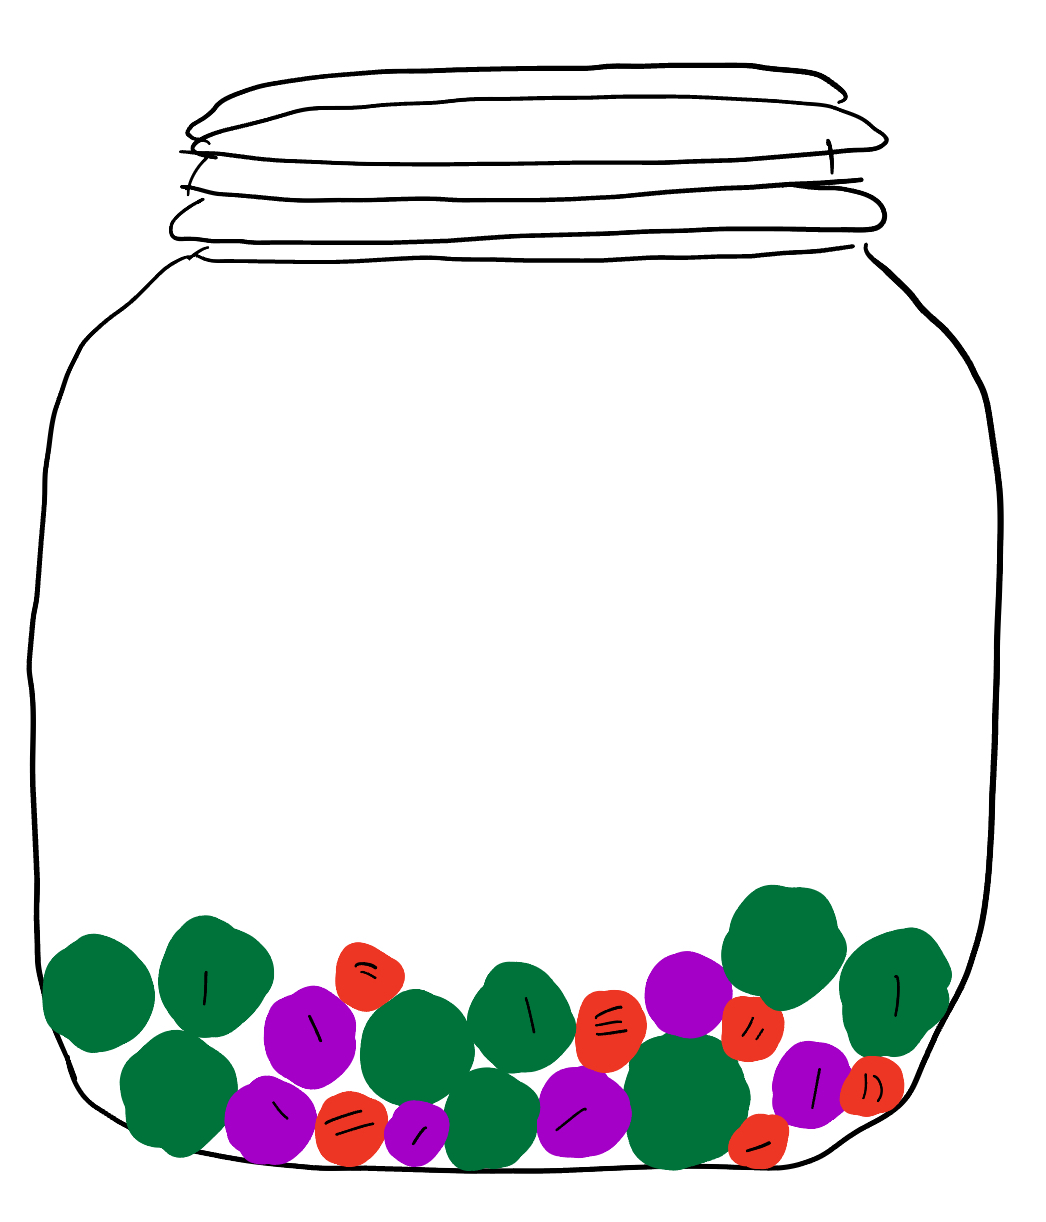
\includegraphics{../IMG_0317.png}

}

\caption{Jar of reading orbs}

\end{figure}%

\subsection{d.}\label{d.-1}

My affective visualization shows a jar containing many orbs. Each orb is
an independent reading session, which is affected by length of reading,
comprehension, and distractions. I took inspiration from the examples
provided of Jill Pelto's paintings. I drew my peice on my iPad. I
started off with a drawing of a jar. I then filled the jar with
different size orbs that represent different sessions of reading. Each
orb is to be different in size, color, and defects on the surface.

\section{Problem 3. Statistical
Critique}\label{problem-3.-statistical-critique}

\subsection{a.}\label{a.-2}

The statistical tests used by the author to address their main research
question are: Welch's t-test, Mann--Whitney's U-test, Kruskal--Wallis
test, Spearman's correlation coefficient by rank test.

\begin{figure}[H]

{\centering 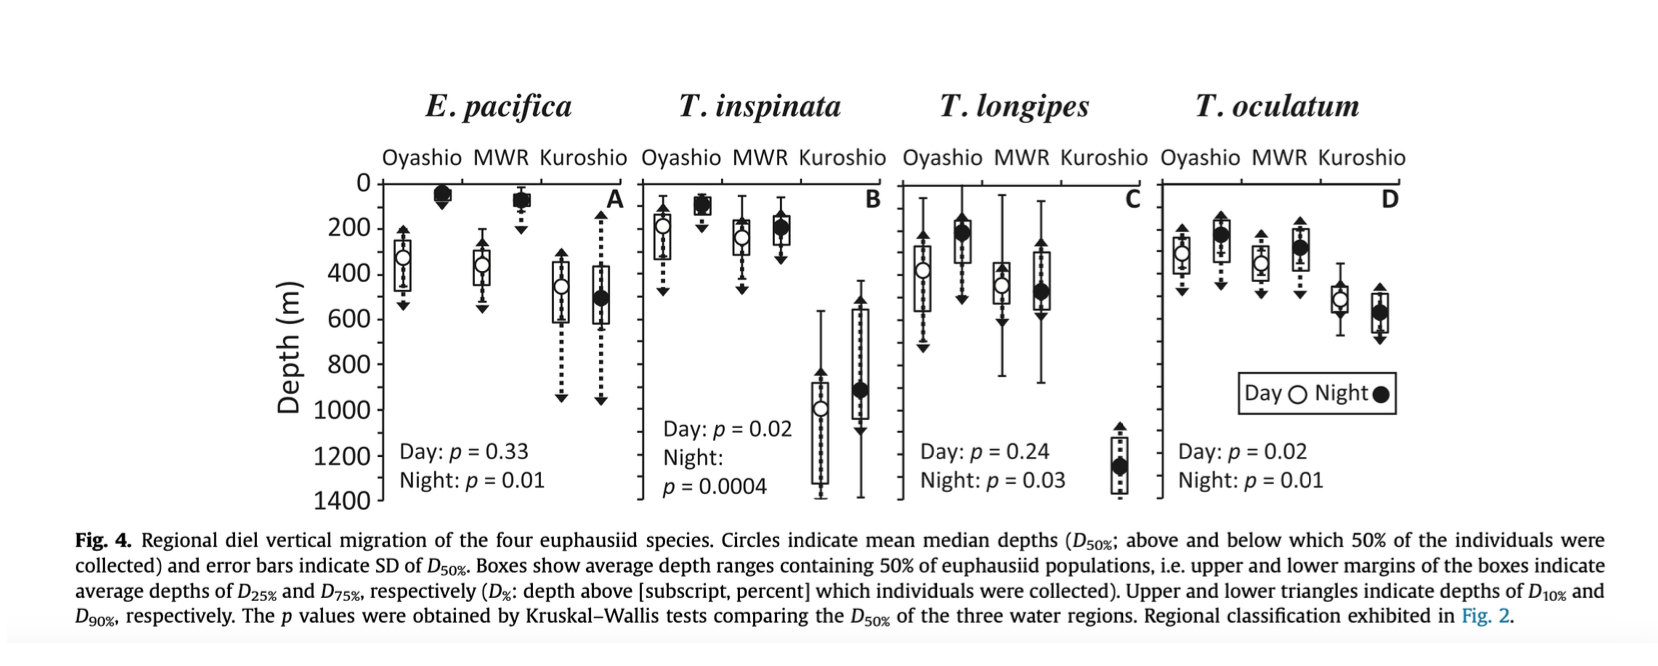
\includegraphics{../statistical_test.png}

}

\caption{Kruskal-Wallis test}

\end{figure}%

\subsection{b.}\label{b.-2}

The author clearly represents their statistics in the figure, with well
labeled axes and depth scale that increases downwards. Each of the four
species include test statistics such as medians, standard deviations,
interquartile ranges, and depth extremes. P-values from Kruskal--Wallis
tests are clearly displayed, making statistical comparisons across
regions clear and easy to interpret.

\subsection{c.}\label{c.-2}

The author handles visual clutter well by using distinct, consistent
symbols (open circles, closed circles, triangles, box plots) and
seperating each species into their own panel. The data:ink ratio is
high, but the visual elements have meaningful information (depth ranges,
medians, p-values). Overall, this figure is information dense yet clear
and visually effective.

\subsection{d.}\label{d.-2}

I would recommend adding a sample size for each box plot in the legend,
which can help readers evaluate the variability of the summary
statistics. Instead of using open and closed circles to differentiate
between night and day, I would recommend adding color to enhance the
immediate visual distinction without overwhelming the figure, I would
add clarity in the legend, specifically the triangles and boxes to make
it easier to understand what they represent. Lastly, a summary of the
findings at the bottom of the figure that quickly helps the reader grasp
significant patterns without having to interpret each subplot
individually.




\end{document}
